\documentclass{article}
\usepackage{amsmath}
\usepackage{graphicx}
\usepackage{float}
\usepackage{geometry}
\geometry{margin=1in}

\title{Assignment 5}
\author{ESCI 5331 \\ Jenny Huang}
\date{}

\begin{document}

\maketitle

\section*{2: Confined pump test}
#TO DOOOOOO
\section*{3: 1D Groundwater Flow}
\begin{enumerate}[label=\alph*]  
    \item Because this is steady-state and the boundary head values are held constant, the boundary head values do not change with changing K. 
    Thus, overall \frac{dh}{dz} is the same for all scenarios. 
    However, flux will change because flux is also dependent on conductivity (or effective conductivity K_{eff} when consolidating multiple layers): 
    \[
    q = -K\frac{dh}{dz}
    \]
    The greater K, the greater the flux. In scenarios ii - iv, K_{eff} = 4.5 m/s (since ordering of layers does not matter for calculating K_{eff}). Therefore, flux is the same. 
    Because K_{eff}^i = 6 m/s, the flux will be greater in scenario i than the other scenarios. 
    
    \item Head profiles for the four different configurations:
    \begin{figure}[H]
        \centering
        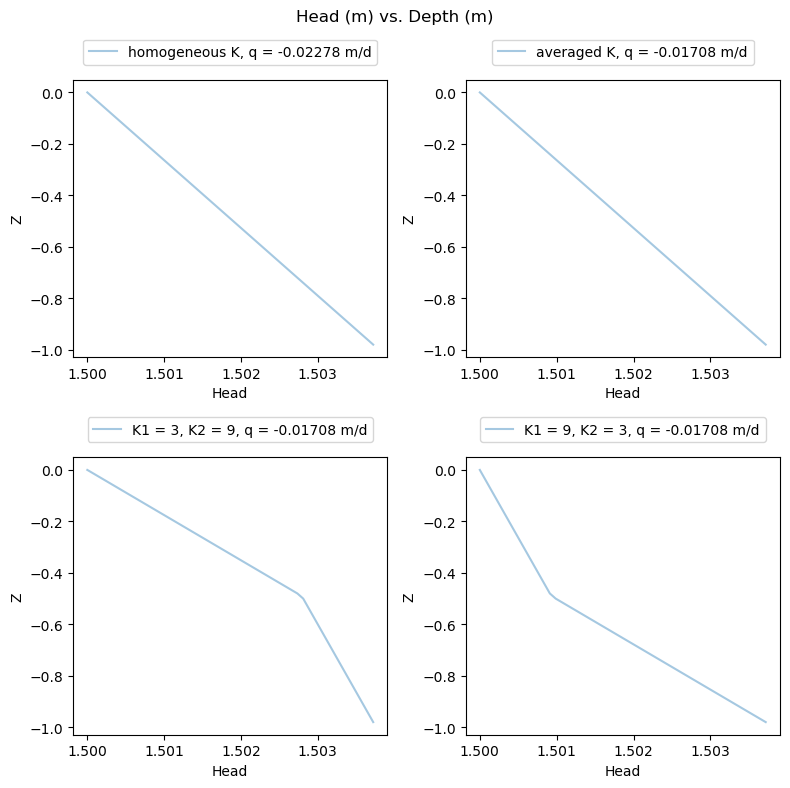
\includegraphics[width=0.5\textwidth]{model_runs/hw5_1d_all_cases_separate.png}
        \caption{1D flow for varying conductivity configurations}
    \end{figure}
    \begin{figure}[H]
        \centering
        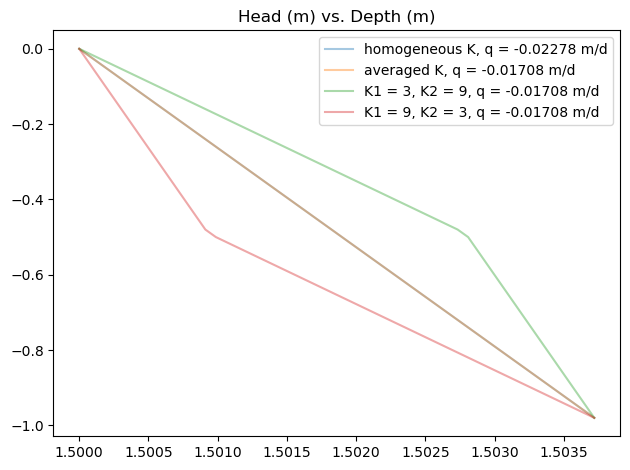
\includegraphics[width=0.5\textwidth]{model_runs/hw5_1d_all_cases.png}
        \caption{1D flow comparison}
    \end{figure}
    \item See above for Darcy flux. The homogeneous case with K = 6 m/d has the highest Darcy flux. 
\end{enumerate}
\section*{4: 2D Groundwater Flow}
\begin{figure}[H]
    \centering
    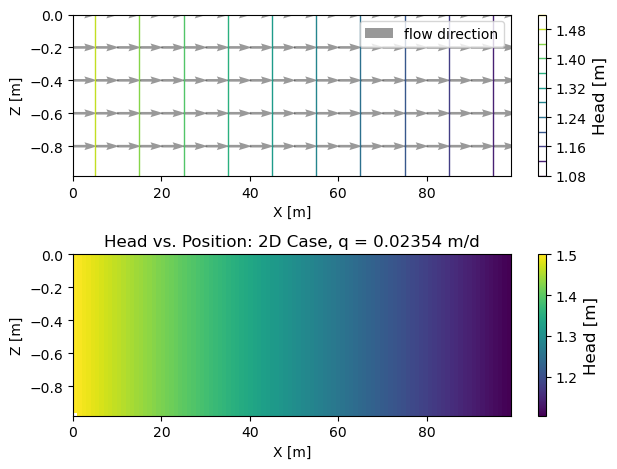
\includegraphics[width=0.5\textwidth]{model_runs/2d_case.png}
    \caption{2D flow}
\end{figure}
\section*{5: Recharge}
Adding recharge into the model changes the distribution of head, with a steeper gradient on the right side of the profile.
\begin{figure}[H]
    \centering
    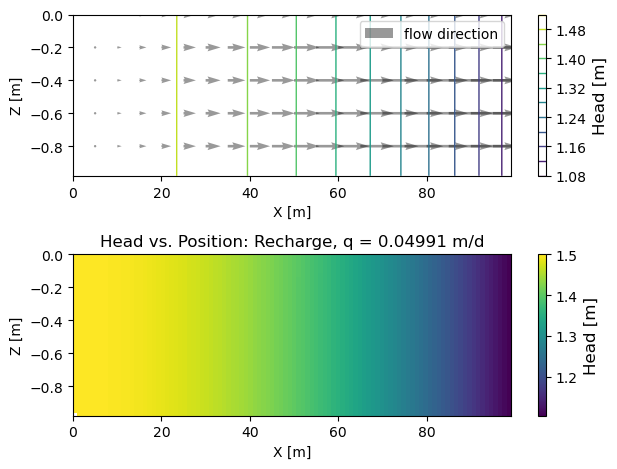
\includegraphics[width=0.5\textwidth]{model_runs/2d_recharge.png}
    \caption{2D flow with recharge}
\end{figure}